
\section{The \app Framework Overview}

\begin{figure*}[tbp] \centering
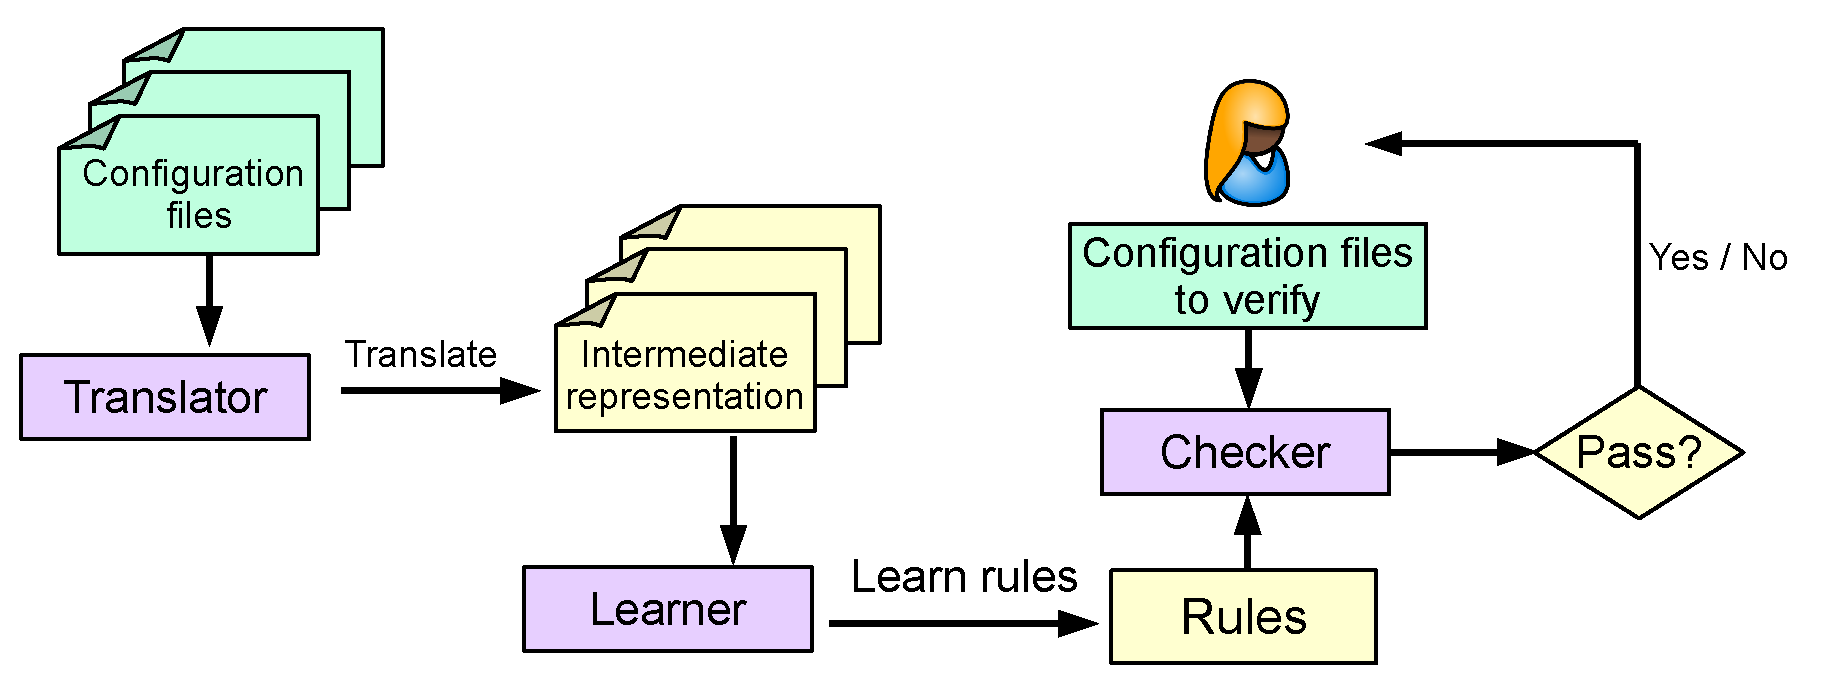
\includegraphics[width=0.88\textwidth]{figs/overview}
\caption{\app's workflow. The green components represent configuration 
  files, including both sample configuration datasets and users' input
  configuration files to verify. 
  The purple components are the modules of \app.
  Because template DB is not necessarily used, we use dashed
  arrow between it and the learner.
  Red boxes are sub-modules within the checker.
  The yellow components are results generated by \app's modules.}
\label{fig-overview}
\end{figure*}

We propose \app, an automatic verification framework for 
software configuration files.
In particular, \app can solve many sophisticated 
configuration errors (\eg, ordering errors, missing entry errors 
and fine-grained value correlation) that previous efforts cannot 
detect. As depicted in Figure~\ref{fig-overview}, 
a typical \app verification workflow has three steps:
translation, learning and checking. In this section, we briefly
describe how does each step work.

\para{Initial phase.}
We start with the assumption 
that we are given a number of (not necessarily correct) 
configuration files belonging to the same system, 
such as MySQL or Apache. 
These given files follow similar patterns, which we exploit
in a learning algorithm to build rules that
describe a language model for the files.

\para{Translator.}
The translator module first parses the input sample 
dataset (containing both configuration files and system environment
information), and then transforms them to a more structured
and typed intermediate representation.
When we run type inference on a configuration file, 
the type of a variable cannot always be fully determined from 
a single value.
We address this problem 
by introducing so called {\em probabilistic types}.
Rather than giving a variable a single type, 
we assign several types with their probability distributions. 
We can later use these more structured files
as a training set to learn the rules. 

\para{Learning.}
The input of learner is a set of files that have been translated
into well-structured and typed representations.
The learner module employs a collection of learning algorithms
to generate various rule and constraints,
potentially used to handle different types of configuration errors.
These rules are the output of the learner, and will be 
used by the checker to detect errors.
By combining the translated representations and the learned
rules together, we already build a language model for
configuration verifications.
Because the translator outputs probabilistic typed entries,
the learner is responsible for determining a type for each entry.

Different from previous efforts, \eg, EnCore~\cite{zhang14encore},
which needs users or developers to provide explicit templates,
\app's learner encodes some predefined error-patterns 
to generate rules. 
As an illustration of a simple rule that we can learn,
consider an encoded pattern $X_1 \le X_2$, where $X_1$ and $X_2$ are
integer variables. The learner may derive the rule stating that
$\texttt{mysql.max\_persistent} \le \texttt{max\_connections}$. 
There is a classification and taxonomy of configuration errors in the 
existing work on automated configuration troubleshooting%
~\cite{yin11anempirical, configdataset}. 
Each class is looked as an error-pattern 
that \app should handle: we consider integer constraints, 
ordering errors, typing errors, correlation errors, etc.
\ennan{I do know we are using in some sense templates, but
we should use pattern or some words to persuade we are 
using an implicit ``templates''; otherwise, too similar 
to what EnCore did.}

Although the learner does necessarily rely on templates,
\app still offers a database to contain many templates,
as shown in Figure~\ref{fig-overview}.
Some of these templates are responsible for offering
specific system executional environment information.
It is widely known that any existing learning algorithm cannot
derive rules checking environment violation, \eg,
whether current account is the owner of a certain path.
In order to deal with comprehensive misconfiguration problems,
the learner needs a template DB to provide environment information,
thus detecting system environment-related configuration errors.

\para{Checking.}
The checker is used to detect the rule violations in the configuration
files of interest. The inputs of checker are the learned rules 
and the target configuration file to verify.
Its outputs a report (as shown in $\S$\ref{sec-motiv}) about 
whether it finds any error, \eg, rule violations, or a suspicious value.
As shown in Figure~\ref{fig-overview},
there are two sub-modules in the checker. They are responsible for
checking rule violations and suspicious values, respectively.
\ennan{I really wanted to say we are using MaxSMT to check and rank
these errors ...}
In our experience, we find learned rules can be significantly reused
to check different configuration files, thus improving our usability.  
